\documentclass[10pt,twocolumn,letterpaper]{article}

\usepackage{algorithmicx}
\usepackage{algorithm}
\usepackage{booktabs}
\usepackage{cvpr}
\usepackage{graphicx}
\usepackage{color, colortbl}
\usepackage{algpseudocode}
\usepackage{booktabs}
\usepackage{hyperref,url}


% List labels
\usepackage{scrextend}
\addtokomafont{labelinglabel}{\sffamily}

\renewcommand{\algorithmicrequire}{\textbf{Input:}}
\renewcommand{\algorithmicensure}{\textbf{Output:}}
\renewcommand{\thefootnote}{$\star$}

\cvprfinalcopy % *** Uncomment this line for the final submission

\usepackage{footmisc} % Daggers for author notes
\DefineFNsymbols{mySymbols}{{\ensuremath\dagger}{\ensuremath\ddagger}\S\P
   *{**}{\ensuremath{\dagger\dagger}}{\ensuremath{\ddagger\ddagger}}}
\setfnsymbol{mySymbols}

% Colors for highlighting tables
\definecolor{Gray}{gray}{0.9}

% Pages are numbered in submission mode, and unnumbered in camera-ready
%\ifcvprfinal\pagestyle{empty}\fi
\setcounter{page}{1}
\begin{document}

%%%%%%%%% TITLE
\title{Parallel stability-based \texttt{k-means}$^\star$}

\author{
    Jason Poulos\thanks{\href{mailto:poulos@berkeley.edu}{\nolinkurl{poulos@berkeley.edu}}}
    \hspace{10mm}
    Emin Arakelian\thanks{\href{mailto:emin@berkeley.edu}{\nolinkurl{emin@berkeley.edu}}}
    \hspace{10mm}
    Fadi Kfoury\thanks{\href{mailto:fadi.kfoury@berkeley.edu}{\nolinkurl{fadi.kfoury@berkeley.edu}}}
    \vspace{15mm}
}

\maketitle
%\thispagestyle{empty}

%%%%%%%%% ABSTRACT
\begin{abstract}
Abstract...
\end{abstract}

\footnotetext[1]{The code used for this project is available on Github: \url{https://github.com/plumSemPy/parallel_kmeans}.}

%\linenumbers

%% main text
\section{Introduction} \label{section:Intro}

Unsupervised learning is a branch of machine learning that infers patterns from data that has no labels. \texttt{k-means} is a popular unsupervised algorithm for finding clusters and cluster centers in data. The goal is to choose $k$ cluster centers to minimize the total squared distance between each data point and its closest center. Given $k$ initial centers chosen uniformly at random from the data points, \texttt{k-means} alternates between two steps until convergence: (\textit{assignment step}) each point is assigned to the nearest cluster center and; (\textit{update step}) each center is recomputed as the center of mass of all points assigned to it.

\texttt{k-means} is NP-hard, and can be solved in time  $O (n^{dk +1} \log n)$, where $n$ is the number of points in $d$ dimensions. While it's hard to parallelize \texttt{k-means} itself due to its sequential nature, researchers can find shortcuts in the algorithm, or run numerous \texttt{k-means} instances on sub-samples to evaluate the stability of clustering. Our project compares sequential and parallelized versions of the stability-based method. 

After briefly reviewing other parallel implementations of \texttt{k-means} in Section~\ref{section:rw}, we describe the stability-based method and its parallel implementation in Section~\ref{section:stability}. We then describe experiments and results in Section~\ref{section:experiments}. Finally, we draw conclusions in Section~\ref{section:Con}.

\section{Related work}  \label{section:rw}
\paragraph{\texttt{k-means++}} chooses only the first cluster center uniformly at random; subsequent centers are selected from the data points, weighed by a probability proportional to its contribution to the overall error. This initialization algorithm is shown to obtain a set of initial centers that is close to the optimum solution \cite{arthur2007}. 

\paragraph{\texttt{k-means||}} \texttt{k-means++} is ill-suited for massive data because it makes $k$ sequential passes over the data points in order to obtain the initial centers. Bahmani et al. \cite{bahmani2012} propose a method of parallelizing the initialization that reduces the number of passes, which they call \texttt{k-means||}. Instead of sampling a single point in each pass, \texttt{k-means||} samples $O(k)$ points and repeats for $O (\log n)$ rounds.

\section{Stability-based method} \label{section:stability}

Ben-Hur et al. \cite{ben2001} propose an algorithm that uses stability of clustering with respect to perturbations such as sub-sampling as a means of defining meaningful partitions.  Computing the stability measure is the bottleneck, so parallelizing the algorithm will involve enhancements to re-use parts of the computations and avoid storing/writing the full matrix multiplication for computing the measure.

\subsection{Parallel implementation} 

\section{Experiments} \label{section:experiments}

We compare the algorithms using data from a dialect survey, which includes linguistic binary encoded responses \cite{vaux2003}. The linguistic survey data can be used to study dialectometry, or linguistic variations with spatially determined distributions. These data, which feature questions on lexical choice and pronunciation, can be used to identify dialect areas and to determine whether linguistic diversity is isolated or a transitional area between areas of linguistic uniformity. 

We implement the serial and parallel stability-based methods in Python and run all implementations on Edison. Performance is evaluated on three dimensions -- clustering cost, running time, and space complexity -- for different values of $k$.

\begin{figure*}[htbp] 
   \centering
   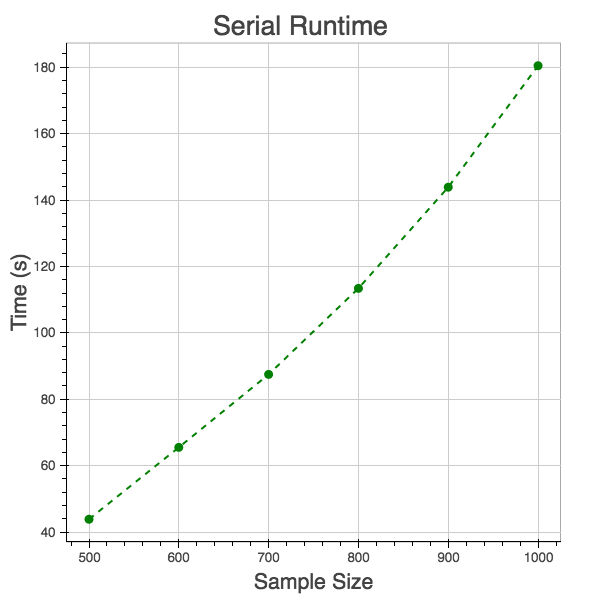
\includegraphics[width=0.8\textwidth]{./figure/serial.png}
   \caption{Serial code complexity.}
   \label{fig:serial}
\end{figure*}

\subsection{Choice of clusters} 

Figure~\ref{fig:cumulative_similarity} plots the overlay of the cumulative distributions of the similarity scores for varying values of $k$. We see that the distribution of similarities for each $k$ are similar and close to 1. A choice of any number of clusters between $2 \leq k \leq 10$ would be reasonable;  however, the choice of $k=2$ appears to be the optimal choice. At $k=2$, the cumulative distribution converges toward unity faster than the other distributions. 

\begin{figure*}[htbp] 
   \centering
   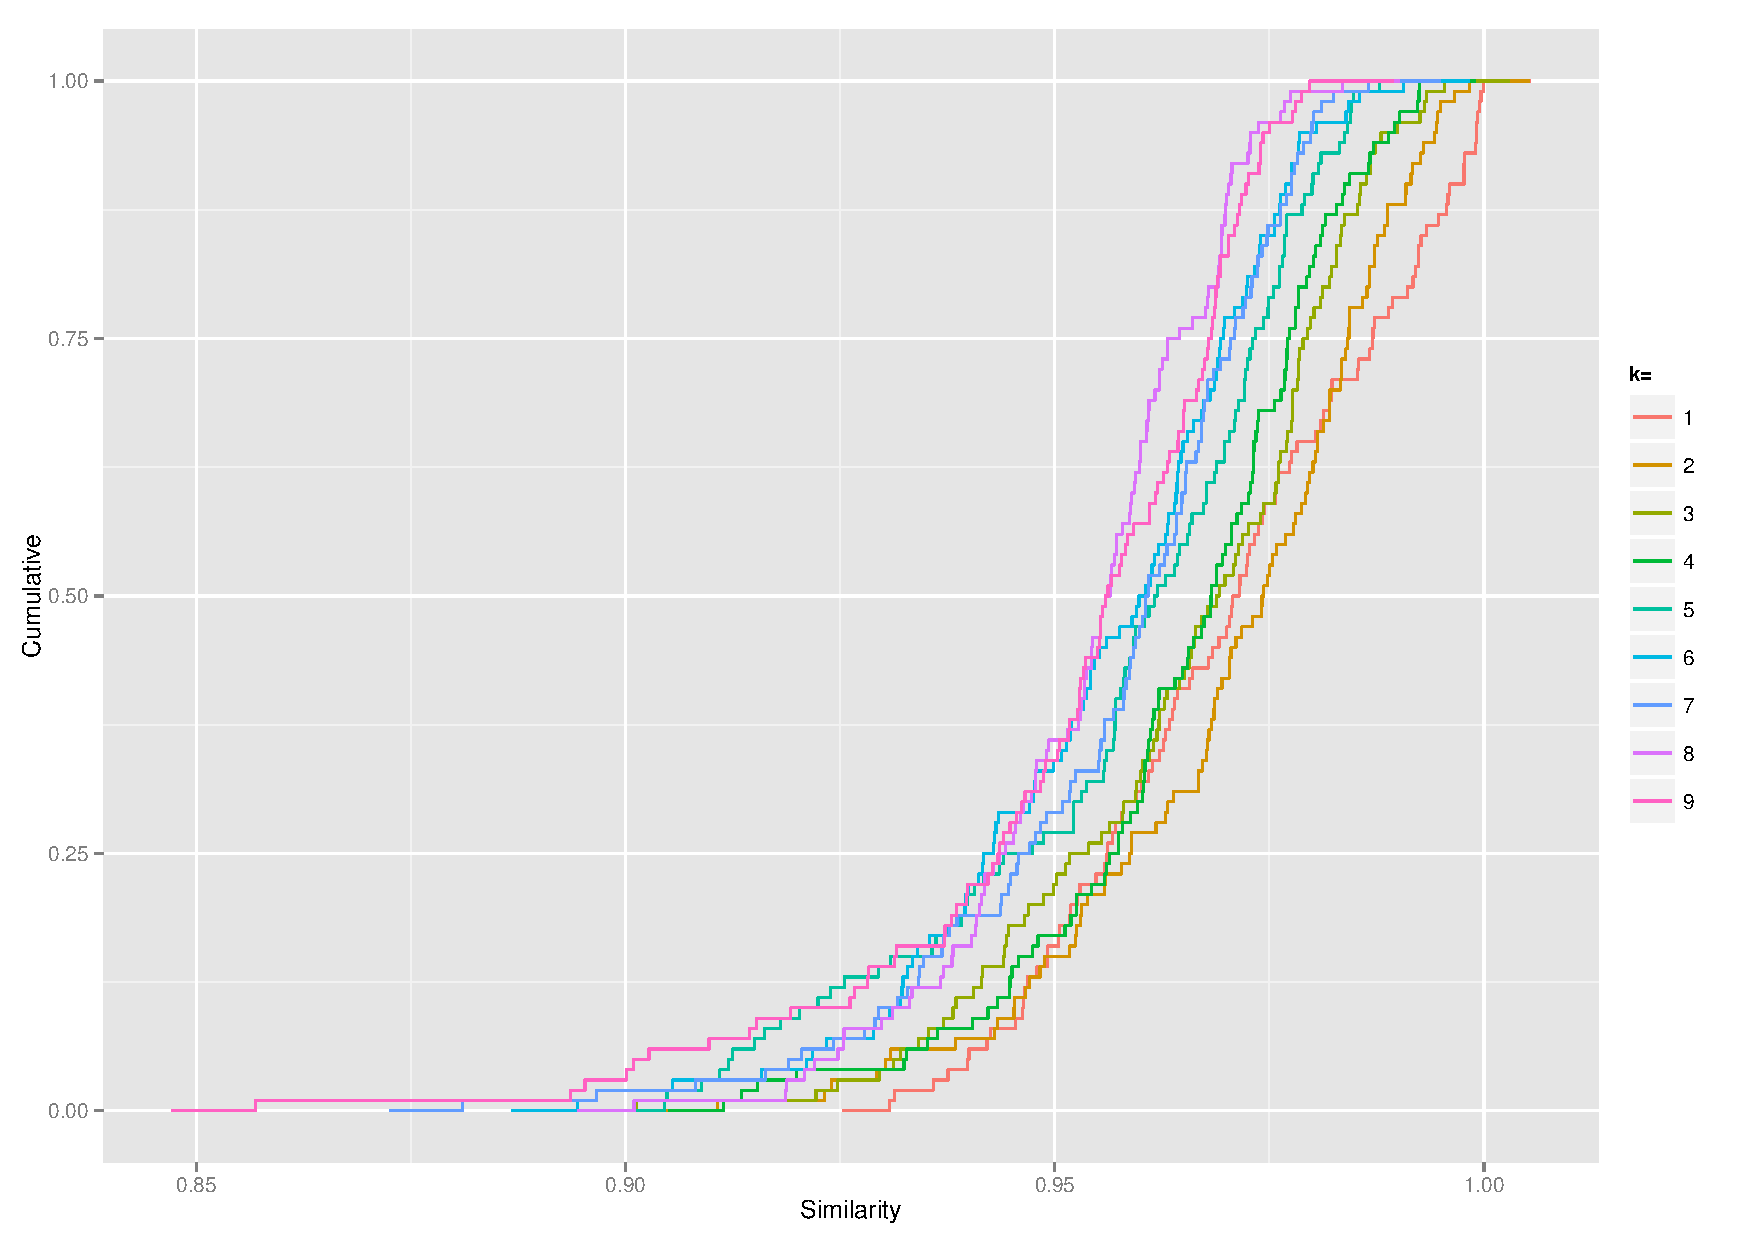
\includegraphics[width=0.8\textwidth]{./figure/cumulative_similarity.pdf}
   \caption{Overlay of the cumulative distributions of the correlation similarity measure for $n=100$ runs and increasing values of $k$}
   \label{fig:cumulative_similarity}
\end{figure*}

In order to determine the appropriate number of clusters, Figure~\ref{fig:scree_plot} Figure 3 plots the within--group sum of squares for $k \leq 25$ clusters. We choose $k=16$ clusters because the within--groups sum of squares (WSS) do not decrease much after $k=16$. While the location of the ``elbow''  is ambiguous, it is clear that the greatest difference in reducing WSS happens when $k$ moves from 1 to 2 and that the reduction of WSS diminishes after $k=2$. 

\begin{figure*}[htbp] 
   \centering
   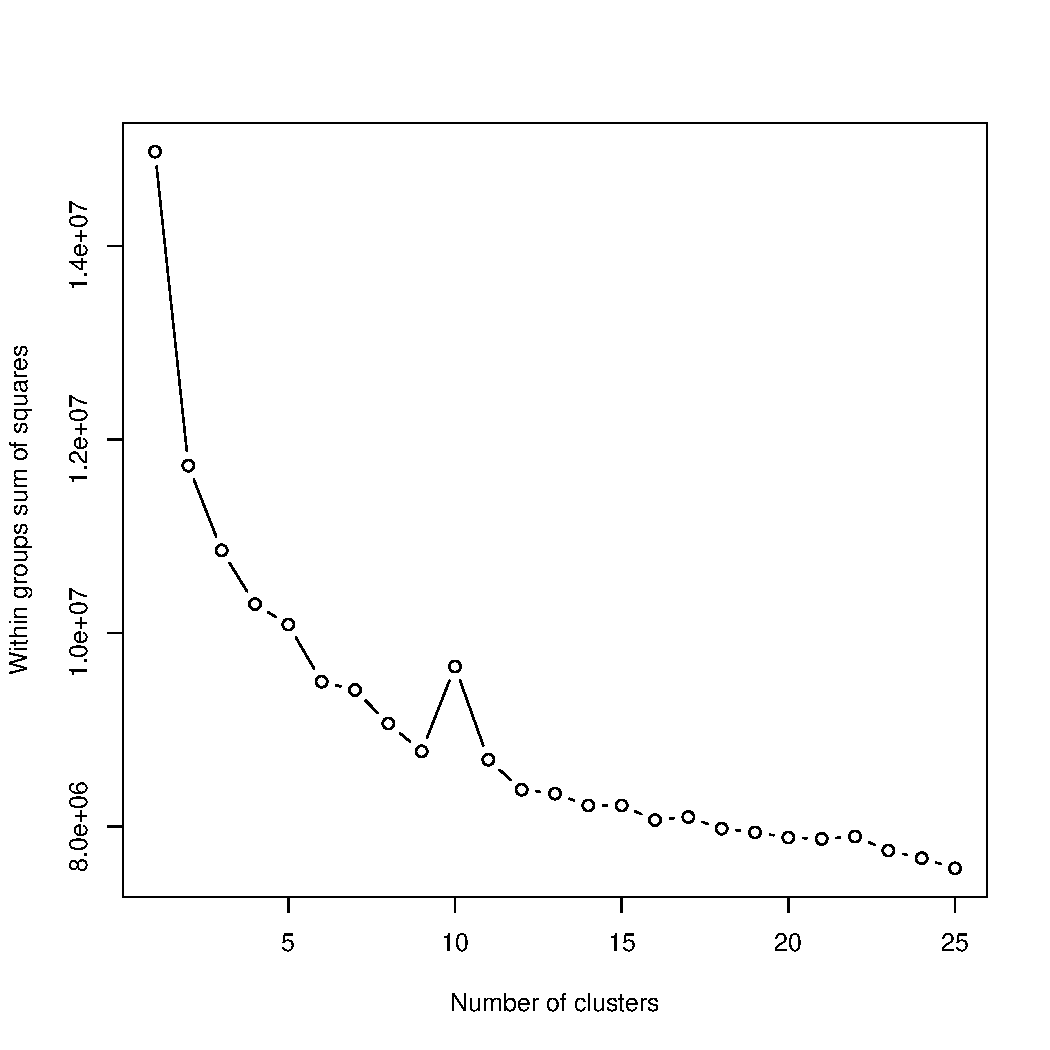
\includegraphics[width=0.8\textwidth]{./figure/scree_plot.pdf}
   \caption{Sum of squared error scree plot of linguistic data. The location of the elbow in the plot suggests a suitable number of clusters for the k--means.}
   \label{fig:scree_plot}
\end{figure*}

\section{Conclusion} \label{section:Con}


%\section*{Acknowledgments}

{\small
\bibliographystyle{ieee}
\bibliography{refs}
}

\end{document}
